\mysection{ОБЗОР ПЛАТФОРМЫ ДЛЯ РАЗРАБОТКИ И~ПРОЕКТИРОВАНИЕ ВЕБ-ПРИЛОЖЕНИЯ}

\subsection{Платформа для разработки}

Разработка приложения будет осуществляться на платформе продуктов компании Emlid \cite{Emlid}: ГНСС модуля Reach \cite{Reach} и~ГНСС приёмника Reach~RS \cite{ReachRS}. Основой данных устройств являются вычислительный модуль Intel Edison и~плата, на которую установлен ГНСС модулю компании u-blox. Intel Edison работает под управлением GNU/Linux, что позволяет использовать многочисленные средства разработки, доступные для дистрибутивов данной операционной системы. \par

При разработке приложения на платформе указанных выше устройств важно учитывать следующий факт: несмотря на то, что Reach и~Reach~RS созданы на базе одного и~того же вычислительного модуля и~используют одинаковые приёмники u-blox, имеется ряд существенных различий в~аппаратном обеспечении данных устройств \cite{Reach, ReachRS}. Различия Reach и~Reach~RS, которые необходимо учесть при создании веб-приложения, указаны в~таблице \ref{tab:reach-vs-reachrs}.

\ctable[
  pos=h!,
  caption={Различия Reach и~Reach~RS},
  label={tab:reach-vs-reachrs}
]{|l|*{2}{>{\centering\arraybackslash}m{2.3cm}|}}{}{
  \toprule
  \multicolumn{1}{|c|}{\textbf{Техническая/функциональная особенность}} & \textbf{Reach} & \textbf{Reach~RS} \\
  \midrule
  Встроенная батарея & нет & да \\
  \midrule
  Встроенная антенна & нет & да \\
  \midrule
  Встроенное радио & нет & да \\
  % \midrule
  % Физическая кнопка на корпусе & нет & да \\
  \midrule
  Возможность управления фотокамерой & да & нет \\
  \bottomrule
}

Наличие (отсутствие) тех или иных возможностей у~Reach или Reach~RS отразится на клиентской части разрабатываемого решения в~виде специфических форм и~элементов интерфейса, отображение которых будет зависеть от того, на каком из устройств запущено приложение.

\subsection{Общая архитектура приложения}

\subsubsection{Задачи и~требования}

Для создания общей архитектуры приложения необходимо определить наиболее важные идеи, задачи и~требования, предъявляемые к~разрабатываемому продукту. \par

Важно отметить, что в~следующем далее списке присутствуют пункты, которые касаются лишь разработчиков программных компонентов, отвечающих за взаимодействие с~RTKLIB, системными утилитами и~различными аппаратными компонентами Reach и~Reach~RS. Данные модули и~детали их разработки выходят за рамки рассматриваемой работы, но являются чрезвычайно важными для понимания общей структуры приложения. \par

Разрабатываемое приложение должно:

\begin{dashitemize}
  \item \textbf{Осуществлять запуск приложений RTKLIB в~управляемых контейнерах}. Надёжным и~простым способом организации взаимодействия с~приложениями RTKLIB является их запуск в~управляемых контейнерах. При данном подходе необходимые утилиты будут работать так же, как если бы пользователь запускал их в~терминале. \par

  Используя подобный подход, становится возможно организовать взаимодействие веб-приложения с~необходимыми программами таким образом, что:

  \begin{dashitemize}
    \item не требуется вмешательство в~исходный код RTKLIB;
    \item облегчается поддержка совместимости с~новыми версиями программного комплекса;
    \item разрабатываемый продукт остаётся независим от изменений в~кодовой базе RTKLIB. 
  \end{dashitemize}

  \item \textbf{Иметь клиентскую часть, представленную в~виде одностраничного приложения}. Основываясь на выводах, сделанных в~разделе 1, было принято решение реализовать клиентскую часть разрабатываемого решения в~виде одностраничного приложения. \par

  Как показал проведённый обзор, данный подход в~настоящее время является одним из самых популярных решений для создания веб-интерфейсов, предназначенных для управления такими устройствами, как Reach или Reach~RS.

  \item \textbf{Поддерживать передачу данных по протоколу WebSocket}. Для создания отзывчивого интерфейса веб-приложения и~обеспечения лучшего пользовательского опыта б\`{о}льшую часть взаимодействий клиентской части с~сервером следует организовать с~помощью асинхронных запросов и~сообщений. \par

  Наиболее удачным решение для разрабатываемого приложения является протокол WebSocket. Создавая на клиентской части веб-приложения слушателей определённых событий, становится возможно организовать отображение различной информации в режиме реального времени без постоянных опросов сервера.
\end{dashitemize}

\subsubsection{Основные модули}

Перечислим основные модули приложения (рис.~\ref{fig:raw-system-architecture}):

\begin{alphitemize}
  \item Серверная часть
  \begin{alphitemize}
    \item WebSocket сервер
    \item Модуль взаимодействия с~RTKLIB
    \item Демоны и~сервисы для взаимодействия с~аппаратными компонентами устройства
  \end{alphitemize}

  \item Клиентская часть
  \begin{alphitemize}
    \item WebSocket клиент
    \item JavaScript-приложение
  \end{alphitemize}
\end{alphitemize}

\begin{figure}[h!]
  \centering
  \setlength{\fboxsep}{5pt}
  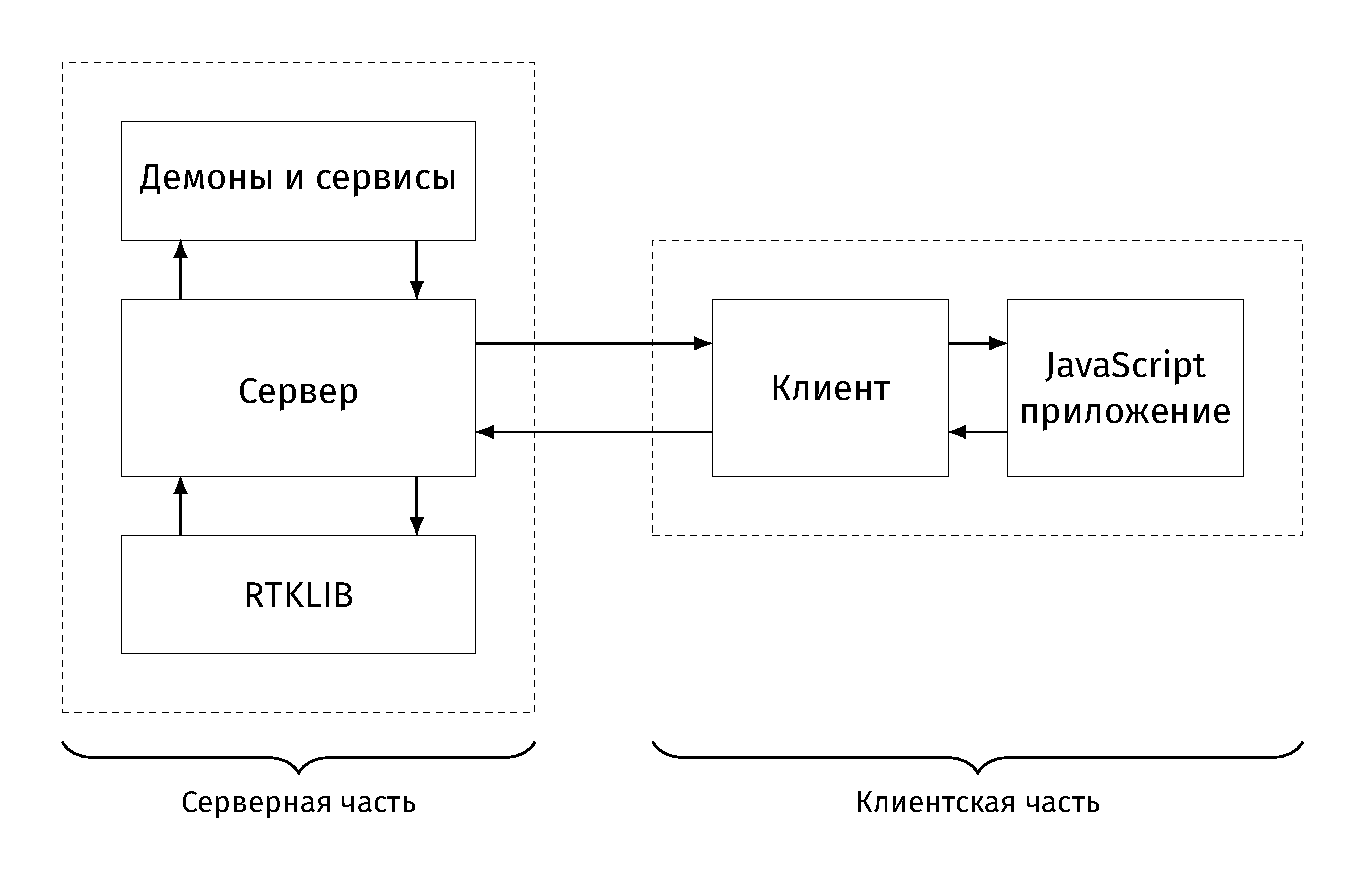
\includegraphics[width=.9\textwidth]{img/tikz/raw-system-architecture/pic}
  \vspace*{12pt}
  \caption{Общая архитектура приложения}\label{fig:raw-system-architecture}
\end{figure}

\subsection{Выбор инструментов разработки}

\subsubsection{Серверная часть приложения}

В~рамках разработки описанного приложения выбор инструментов для написания серверной части приложения зависит не только от возможностей веб-фреймворков, доступных для того или иного языка программирования, но и~от задач, описанных в~подразделе 2.2. Также, важно помнить, что разрабатываемое приложение предназначено для запуска на устройствах с~ограниченными вычислительными ресурсами. \par

Разработчиками серверной части приложения был проведён обзор высокоуровневых языков программирования, часто используемых для разработки веб-приложений. Основными из рассмотренных вариантов были такие популярные языки, как Java, Python, Ruby. \par

% TODO Оформить "переход" к списку наиболее важных библиотек/фреймворков
На основании различных оценок, детали формирования которых выходят за рамки рассматриваемой работы, основным языком для серверной части приложения был выбран Python.

\begin{dashitemize}
  \item Веб-фреймворк Flask
  \item pexpect
  \item GeoPandas
\end{dashitemize}

\subsubsection{Клиентская часть приложения}

% TODO Дополнить содержание + исправить порядок абзацев
Как уже было сказано ранее, клиентскую часть разрабатываемого решения было решено реализовать в~виде одностраничного приложения. \par

Для работы с WebSocket была выбрана библиотека Socket.IO [?]. Данный выбор обусловлен не только популярностью библиотеки, но и наличием полной поддержки Socket.IO на серверной части приложения -- для веб-фреймворка Flask существует расширение Flask-SocketIO, позволяющее серверу обмениваться сообщениями с любыми клиентами Socket.IO.

\begin{dashitemize}
  \item HTML + JavaScript
  \item Vue.js + Vuex
  \item Socket.IO
  \item D3
  \item OpenLayers
\end{dashitemize}

\subsection{Детализированная архитектура приложения}

\subsubsection{Подробная архитектура клиентской части приложения}

\subsection{Создание макета веб-приложения}

\subsubsection{Общий вид приложения}

\subsubsection{Детализация интерфейса отдельных модулей приложения}

\begin{dashitemize}
  \item \textbf{Статус}.
  \item \textbf{Изыскания}.
  \item \textbf{Настройки RTK}.
  \item \textbf{Входящие поправки}.
  \item \textbf{Выдача позиции}.
  \item \textbf{Режим базы}.
  \item \textbf{Логирование}.
  \item \textbf{Управление камерой}.
  \item \textbf{Wi-Fi/Bluetooth}.
  \item \textbf{Настройки}.
\end{dashitemize}

\newpage
